% DESCRIBE EXPLORATIONS TO THIS RESEARCH
\begin{figure}[!htp] \centering 
  \centering
  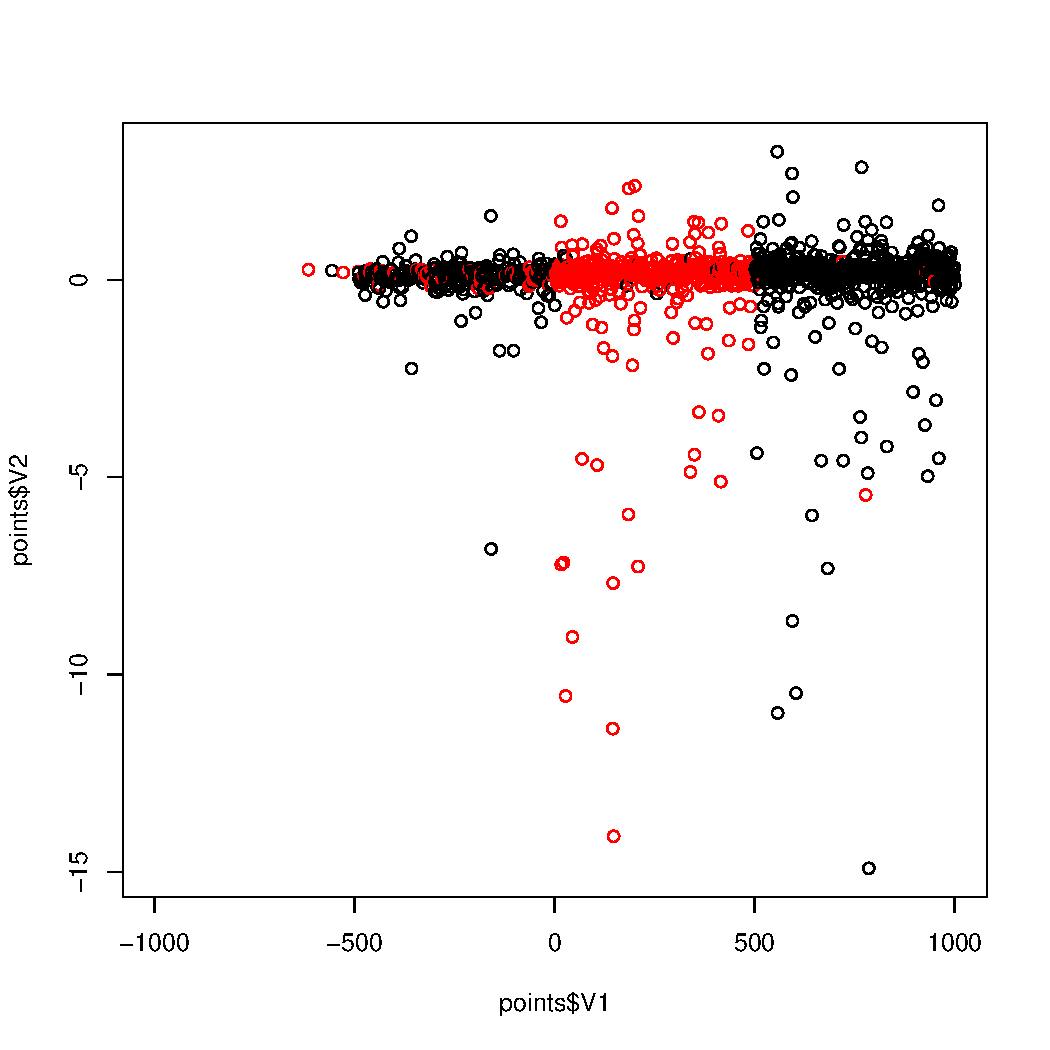
\includegraphics[width=0.8\columnwidth]{assets/pdcl/20newsgrou2fcmsoft-fdcleuclidian.pdf} 
  \caption{Ilustração denotando os
  grupos $g_1,g_2,g_3$ organizados sem sobreposição, para $m = 1$.} 
  \label{fig:newsgroup}
\end{figure}
\begin{figure}[!htp] \centering 
    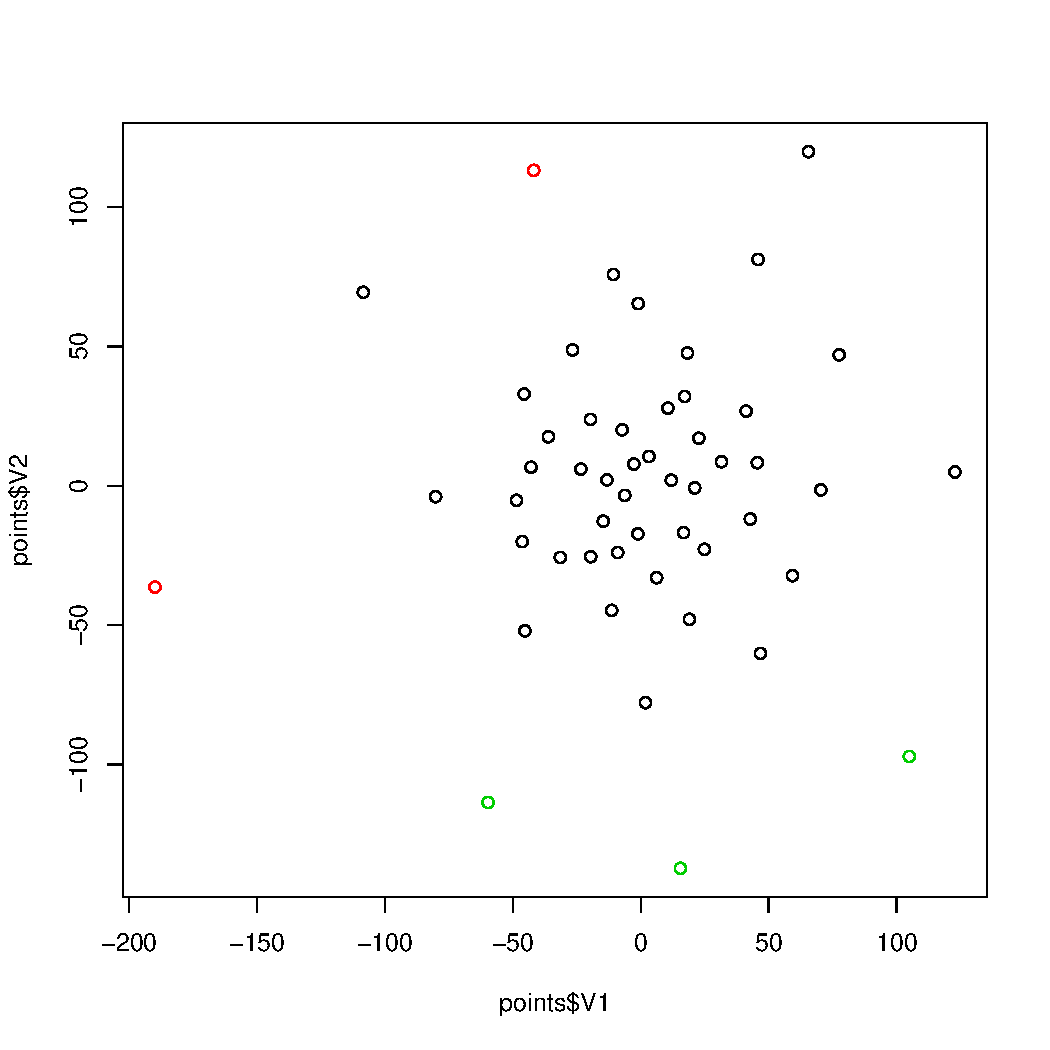
\includegraphics[width=0.8\columnwidth]{assets/pdcl/pfcmmixed-pdcleuclidian.pdf} 
    \caption{Ilustração denotando os
     grupos $g_1,g_2,g_3$ organizados de maneira fuzzy, com sobreposição, quando 
     $m \rightarrow \infty$.}
     \label{fig:mixed_opinosis} 
\end{figure}
